Il seguente codice MatLab contiene la soluzione del problema dell'Es.9 :\\\
	\lstinputlisting[language=Matlab]{Cap_4/Es_9/Es_9.m}
Le seguenti figura mostrano il polinomio di \textit{Lagrange}, al variare del grado \textit{N} del polinomio con $N=2,4,6,8...40$ :
	\begin{figure}[H]
		\label{Cap_4_Es_9_1}
		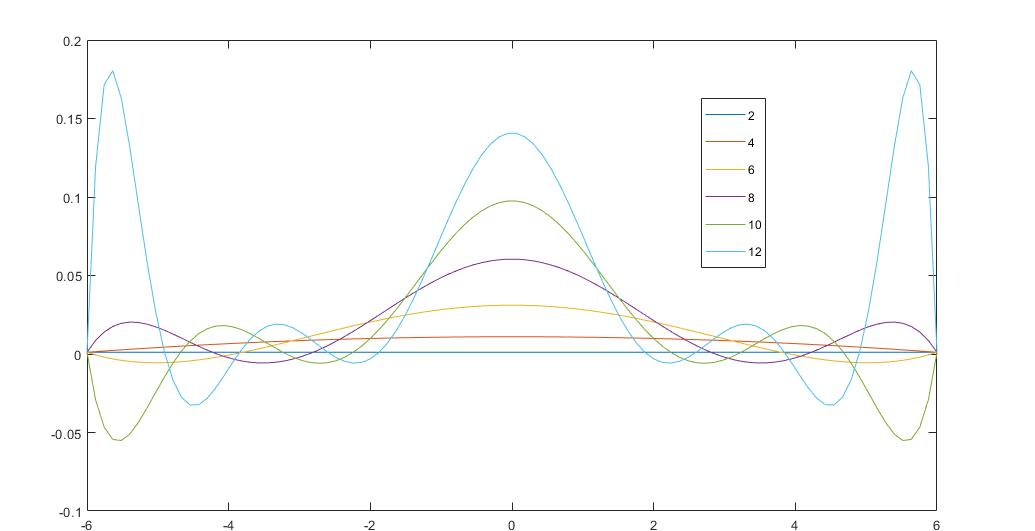
\includegraphics[width=\textwidth]{Plot/Cap_4_Es_9_1}
		\caption*{Polinomio di Lagrange con n° di ascisse $[2,4,6,8,10,12]$}
	\end{figure}
	\begin{figure}[H]
		\label{Cap_4_Es_9_2}
		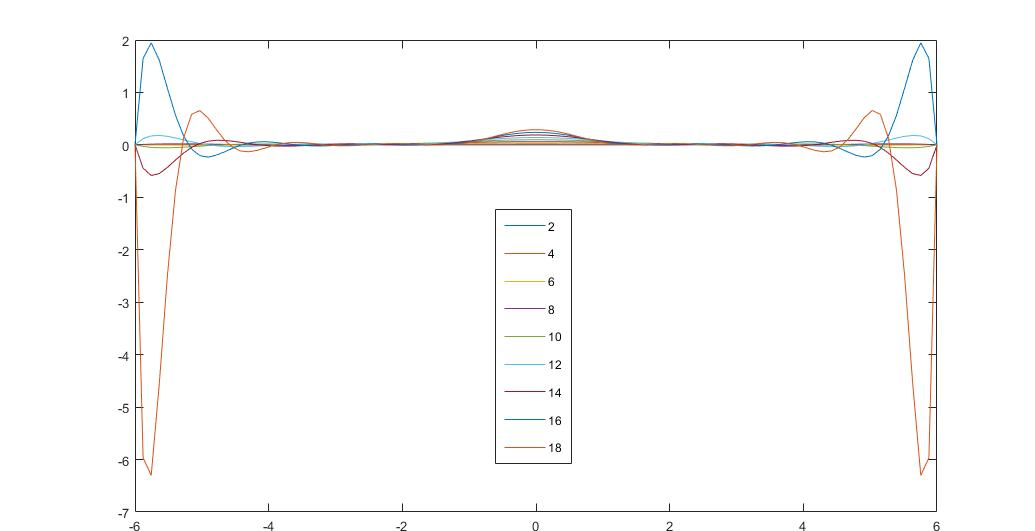
\includegraphics[width=\textwidth]{Plot/Cap_4_Es_9_2}
		\caption*{Polinomio di Lagrange con n° di ascisse $[2,4,6,8,10,12,14,16,18]$}
	\end{figure}
	\begin{figure}[H]
		\label{Cap_4_Es_9_2}
		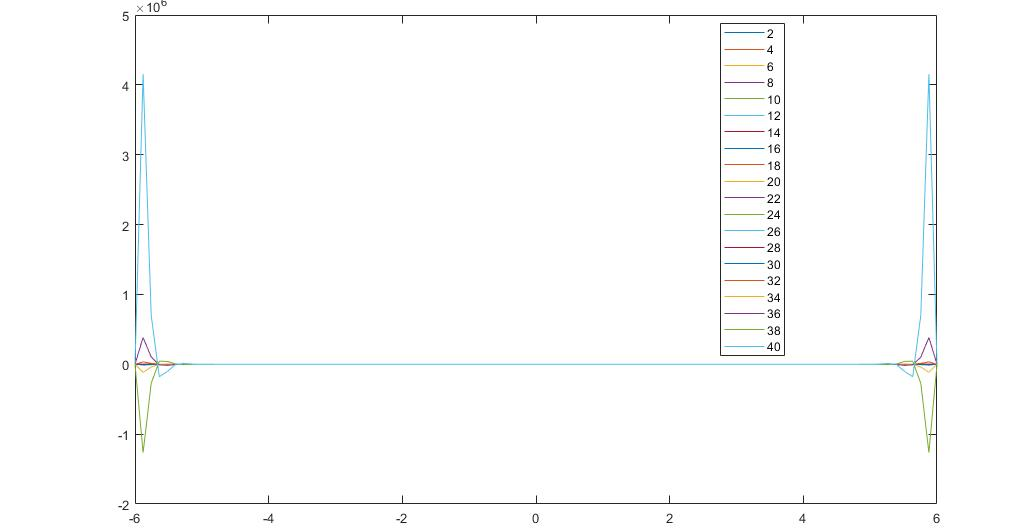
\includegraphics[width=\textwidth]{Plot/Cap_4_Es_9_3}
		\caption*{Polinomio di Lagrange con n° di ascisse $[2,4,6,8,..,40]$}
	\end{figure}
Le seguenti figure mostrano l'andamento della \textit{Spline cubica Naturale} e della \textit{Spline cubica NotAKnot}, al variare del grado \textit{N} del polinomio con $N=2,4,6,8...40$ : 
